\chapter{Vector Analysis}

\section{Vector Algebra}

\subsection{Vector Operations}

\subsection{Vector Algebra: Component Form}

These first two subsections reviews the basics of vectors; for the purpose of these notes, I will assume the reader already has a strong basic understanding of vectors, so they will be left empty.

\subsection{Triple Products}

The output of a cross product $\vec{b}\times\vec{c}$ is a vector, so it can be dotted or crossed with another vector $\vec{a}$ to form a triple product.

The \vocab{scalar triple product} $\vec{a}\cdot(\vec{b}\times\vec{c})$ gives the signed volume of the parallelepiped generated by $\vec{a},\vec{b},\vec{c}$. Therefore,
\begin{claim}
$\vec{a}\cdot(\vec{b}\times\vec{c})=\vec{b}\cdot(\vec{c}\times\vec{a})=\vec{c}\cdot(\vec{a}\times\vec{b})$.
\end{claim}
Notice that we preserved the cyclic order of the vectors in this case; if we flip the order (e.g. $\vec{a}\cdot(\vec{c}\times\vec{b})$), then we obtain the same value with opposite sign. In component form, we have
\[\vec{a}\cdot(\vec{b}\times\vec{c})=\det\begin{bmatrix}
a_x & a_y & a_z\\
b_x & b_y & b_z\\
c_x & c_y & c_z
\end{bmatrix},\]

The \vocab{vector triple product} $\vec{a}\times (\vec{b}\times \vec{c})$ can be simplified by the so-called ``$bac-cab$ rule":
\begin{claim}
$\vec{a}\times(\vec{b}\times\vec{c})=\vec{b}(\vec{a}\cdot\vec{c})-\vec{c}(\vec{a}\cdot\vec{b}).$
\end{claim}
Note that cross-products are not associative, so the order of parentheses matters. By repeated application of this fact, it is never necessary for an expression to contain more than one cross product in any term. For example,
\[(\vec{a}\times \vec{b})\cdot(\vec{c}\times\vec{d})=(\vec{b}\times(\vec{c}\times \vec{d}))\cdot \vec{a}=(\vec{c}(\vec{b}\cdot\vec{d})-\vec{d}(\vec{b}\cdot\vec{c}))\cdot\vec{a}=(\vec{a}\cdot\vec{c})(\vec{b}\cdot\vec{d})-(\vec{a}\cdot\vec{d})(\vec{b}\cdot\vec{c}),\]
where in the first equality we utilized the scalar triple product identity $\vec{a}\cdot(\vec{b}\times\vec{c})=\vec{b}\cdot(\vec{c}\times\vec{a})$.

\subsection{Position, Displacement, and Separation Vectors}

\begin{definition}
Given a coordinate system with origin $\mathcal{O}$, the vector from $\mathcal{O}$ to some point is the \vocab{position vector}
\[\vec{r}:=x\hat{x}+y\hat{y}+z\hat{z},\]
where $(x,y,z)$ are the Cartesian coordinates of the point. 
\end{definition}
Note that the distance from the point to the origin is
\[r=|\vec{r}|=\sqrt{x^2+y^2+z^2}\]
and the unit vector in the direction of $\vec{r}$ is 
\[\hat{r}=\frac{\vec{r}}{r}=\frac{x\hat{x}+y\hat{y}+\hat{z}}{\sqrt{x^2+y^2+z^2}}.\]

\begin{definition}
The \vocab{infinitesimal displacement vector} from $(x,y,z)$ to $(x+dx,y+dy,z+dz)$ is denoted by
\[d\vec{\ell}=dx\hat{x}+dy\hat{y}+dz\hat{z}.\]
\end{definition}
Oftentimes in electrodynamics, we encounter problems involving two points:
\begin{itemize}
    \item A \vocab{source point} $\vec{r'}$, where an electric charge is located,
    \item A \vocab{field point} $\vec{r}$, where we are calculating the electric or magnetic field.
\end{itemize}
In the situation when $\vec{r'}\neq \vec{0}$, it is useful to adopt a shorthand notation for the \vocab{separation vector} from the source point to the field point; we will use the script letter
\[\vec{\scripty{r}}:=\vec{r}-\vec{r'}.\]

\subsection{How Vectors Transform}

What exactly is a vector? You might have learned it as ``a quantity with a magnitude and direction," but this isn't exactly satisfactory...

Perhaps a 3-dimensional vector is simply anything with three real components that combine properly under addition. However, what if we considered some silly example like a barrel with $N_x$ pear, $N_y$ apples, and $N_z$ bananas? Is $\vec{N}=N_x\hat{x}+N_y\hat{y}+N_z\hat{z}$ suddenly a vector? Surely not---what is the direction? What is wrong with it?

The answer is that $\vec{N}$ \textit{doesn't transform properly when you change coordinates}.

In three dimensions, if a $x,y,z$ system is rotated to some $\ol{x},\ol{y},\ol{z}$, system, then the coordinates of some vector $\vec{a}$ undergo a matrix transformation
\[
\begin{bmatrix}
\ol{a}_x\\\ol{a}_y\\\ol{a}_z
\end{bmatrix}=\begin{bmatrix}
R_{xx} & R_{xy} & R_{xz}\\
R_{yx} & R_{yy} & R_{yz}\\
R_{zx} & R_{zy} & R_{zz}
\end{bmatrix}\cdot\begin{bmatrix}
a_x\\a_y\\a_z
\end{bmatrix}\qquad\text{or}\qquad \vec{\ol{a}}=R\vec{a}.,
\]
where $R_{ij}$ are some products of trigonometric functions (or it could simply be any arbitrary linear transformation of $\mathbb{R}^3$). More compactly, we can write it as
\[\ol{a}_i=\sum_{j=1}^3 R_{ij}a_j,\]
where index 1 stands for $x$, etc. 

The components of $\vec{N}$ clearly don't transform in this way.

\begin{definition}
Formally, a \vocab{vector} is any set of three components that transforms in the same manner as a displacement when you change coordinates.
\end{definition}

Therefore, displacement is the \textit{model} for the behavior of all vectors.

\begin{definition}
A \vocab{second-order tesnor} is a quantity with \textit{nine} components: $T_{xx}$, $T_{xy}$, $T_{xz}$, $T_{yx}$,\dots ,$T_{zz}$. These transform with \textit{two} factors of $R$:
\[\ol{T}_{ij}=\sum_{k=1}^3\sum_{\ell=1}^3R_{ik}R_{j\ell}T_{k\ell}.\]
You can also rewrite this in matrix form as $\ol{T}=RTR^T$.
\end{definition}

In general, an $n$th-order tensor has $n$ indices and $3^n$ components (in $\mathbb{R}^3$), and transforms with $n$ factors of $R$. Therefore, a scalar is a tensor of order zero (indeed, note that scalars never change under coordinate changes) and a vector is a tensor of order one.

\section{Differential Calculus}

\subsection{``Ordinary" Derivatives}

Suppose we have a single-variable function $f(x)$. What does the derivative $\frac{df}{dx}$ do?

\begin{moral}
The derivative of a function $df/dx$ tells us how rapidly the function $f$ varies when we change $x$ by a tiny amount $dx$.
\end{moral}

In other words, if $x$ is incremented by an infinitesimal amount $dx$ and $f$ changes by an amount $df$, then the derivative is the proportionality factor:
\[df=\left(\frac{df}{dx}\right)dx.\]
From a geometric perspective, the derivative $\frac{df}{dx}$ gives the \textit{slope} at any point on the graph of $f$ against $x$.

\subsection{Gradient}

That's all well and good for one variable. What about functions of three variables, say temperature $T(x,y,z)$ in $\mathbb{R}^3$? 

How do we generalize the notion of the derivative to functions like $T$? 

We want the derivative to tell us how $T$ changes when we move a tiny distance. However, $T$ may change at a different rate depending on the direction we move in! In a room, nudging $z$ will probably have a much higher affect on the temperature than nudging $x$ or $y$ the same amount.

Fortunately, the situation is not so bad: it turns out that when we zoom in enough, a differentiable function $T$ will always look like a plane, linear in all variables:
\[dT=\left(\frac{\partial T}{\partial x}\right)dx+\left(\frac{\partial T}{\partial y}\right)dy+\left(\frac{\partial T}{\partial z}\right)dz.\]
The proportionality constants are \textit{partial derivatives}, which measure the change in $T$ when you hold all variables constant except for the one in the denominator: therefore, $\frac{\partial T}{\partial x}$ measures the rate of change of $T$ when you move only $x$ by an infinitesimal amount.

This is a rather nice result: we don't need to compute the rate of change of $T$ among all possible directions; three directions $x,y,z$ suffice. 

We can also use it to define another concept. The equation is reminiscent of a dot product:
\[dT=\left(\frac{\partial T}{\partial x}\hat{x}+\frac{\partial T}{\partial y}\hat{y}+\frac{\partial T}{\partial z}\hat{z}\right)\cdot(dx \hat{x}+dy\hat{y}+dz \hat{z}).\]
We give the first vector in this dot product a name:
\begin{definition}
The \vocab{gradient} of a scalar function $T$ is the vector quantity
\[\nabla T:=\frac{\partial T}{\partial x}\hat{x}+\frac{\partial T}{\partial y}\hat{y}+\frac{\partial T}{\partial z}\hat{z}.\]
\end{definition}

Then, $dT=\nabla T\cdot d\vec{\ell}$. Wait... what just happened? This means that if we move by a small vector $d\vec{\ell}$, then the change in $T$ is given by taking the dot product of this small shift vector by the gradient of $T$ at that point. 

Let's dissect this a little more: we can expand the dot product to get
\[dT=\nabla T\cdot d\vec{\ell}=|\nabla T||d\vec{\ell}|\cos\theta,\]
where $\theta$ is the angle between this new gradient vector we just defined and the small shift $d\vec{\ell}$ that we take. Suppose we \textit{fix} the magnitude of $d\vec{\ell}$, so we're always stepping the same tiny amount. Then, if we search various directions by varying $\theta$, notice the \textit{maximum} change in $T$ occurs when $\theta=0$. 

Focusing on this case, we extract the following intuition on what exactly the gradient is:

\begin{moral}
The gradient $\nabla T$ points in the direction of maximum increase of the function $T$. Moreover, its magnitude $|\nabla T|$ gives the rate of increase of $T$ along this maximal direction.
\end{moral}

If we point $d\vec{\ell}$ in the opposite direction of the gradient ($\theta=180^\circ$), then the rate of change is precisely the negative, which makes sense. Also note if we point perpendicular to the gradient ($\theta=90^\circ$), $T$ doesn't change along this direction at all.

Here's a nice picture to keep in your mind: suppose you're on a large, bumpy mountain. We can characterize the surface of this mountain by the \textit{two}-variable function $h(x,y)$ which gives the height of the mountain above any point $(x,y)$ in the plane. Standing at any point $(x,y)$, you can look around and find the direction of steepest ascent---that is the \textit{direction} of the gradient. If you calculate the slope of the mountain in that direction (rise over run)---that is the \textit{magnitude} of the gradient. 

As a person standing on the mountain, if you zoom in enough, you can disregard any large scale bumps in the mountain: it simply looks like a plane; this is what allows the dot product formula $dT=\nabla T\cdot d\vec{\ell}$ to work (with this picture in your mind, reason through the $\theta=180^\circ$ and $\theta=90^\circ$ cases again. This is analogous to the one-variable case, where taking the derivative assumes that when you zoom far in enough on $f$, you get something that looks like a straight line. 

\begin{definition}
We call points where $\nabla T=\vec{0}$ \vocab{stationary points}.
\end{definition}

These can be maximums (summits), minimums (valleys), saddle points (a pass), or ``shoulders."

% \subsubsection*{Problems}

% \prob{1.13} Let $\vec{\scripty{r}}$ be the separation vector from a fixed point $(x',y',z')$ to the point $(x,y,z)$, and let $\scripty{r}$ be its length. Show that
% \begin{enumerate}[(a)]
%     \item $\nabla(\scr^2)=2\vec{\scr}$.
%     \item $\nabla(1/\scr)=-\hat{\scr}/\scr^2$.
%     \item What is the \textit{general} formula for $\nabla(\scr^n)$?
% \end{enumerate}

% \begin{proof}
% We skip to part (c), as (a) and (b) are simply special cases $n=2$ and $n=-1$, respectively. First, note that $\vec{\scr}=(x-x')\hat{x}+(y-y')\hat{y}+(z-z')\hat{z}$. Now,
% \[\nabla(\scr^n)=\frac{\partial \scr^n}{\partial x}\hat{x}+\frac{\partial \scr^n}{\partial y}\hat{y}+\frac{\partial \scr^n}{\partial z}\hat{z}=\sum \frac{\partial \scr^n}{\partial x}\hat{x},\]
% where the sum is over $x,y,z$. Now, note that
% \[\frac{\partial \scr^n}{\partial x}=n\scr^{n-1}\cdot\frac{\partial \scr}{\partial x}.\]
% Noting that $\scr=\sqrt{(x-x')^2+(y-y')^2+(z-z')^2}$, we have that
% \[\frac{\partial\scr}{\partial x}=\frac{1}{2}\cdot \frac{1}{\scr}\cdot (2x-2x')=\frac{x-x'}{\scr}.\]
% Therefore,
% \[\nabla(\scr^n)=n\scr^{n-1}\cdot \sum \frac{(x-x')\hat{x}}{\scr}=n\scr^{n-1}\cdot\frac{\vec{\scr}}{\scr}=\boxed{n\scr^{n-1}\hat{\scr}}.\]
% \end{proof}

% TODO: insert 1.13

\subsection{The Del Operator}

\begin{definition}
We define the $\vocab{del operator}$ as the vector operator
\[\nabla:=\hat{x}\frac{\partial}{\partial x}+\hat{y}\frac{\partial}{\partial y}+\hat{z}\frac{\partial}{\partial z}.\]
\end{definition}

The del operator $\nabla$ is not really a vector; it's more of an instruction. When given a scalar function $T$ to act upon, it produces the gradient $\nabla T$.

Nonetheless, $\nabla$ can mimic the behavior of an ordinary vector in virtually every way, if we translate ``multiply" as ``act upon." It is great notational simplification, even if it's a bit of an abuse. Indeed, we can mimic all three types of vector products:

\begin{enumerate}
    \item On a scalar function $T$, $\nabla$ can act to give the gradient $\nabla T$;
    \item On a vector function $\vec{v}$, via the dot product, to give the \vocab{divergence} $\nabla\cdot \vec{v}$;
    \item On a vector function $\vec{v}$, via the cross product, to give the \vocab{curl} $\nabla\times \vec{v}$.
\end{enumerate}
The following sections will analyze the divergence and curl.

\subsection{The Divergence}

\begin{definition}
The \vocab{divergence} of a vector function $\vec{v}$ is the scalar quantity
\[\nabla\cdot \vec{v}=\frac{\partial v_x}{\partial x}+\frac{\partial v_y}{\partial y}+\frac{\partial v_z}{\partial z}.\]
\end{definition}

The name \textit{divergence} is well-chosen: $\nabla\cdot\vec{v}$ is a measure of how much the vector field $\vec{v}$ spreads out (i.e. diverges) from a given point. 

Imagined a lake with streams and eddies where $\vec{v}$ represented the velocity of the water at any given point. If you drop some particles into the lake at any given point, if they spread out, that's a point of positive divergence, while if they collect together, that's a point of negative divergence. The points of positive divergence are sources, while the points of negative divergence are sinks. (This analogy is not perfect, since water is generally incompressible, i.e. has zero divergence; however, you can imagine there are literal underwater faucets or drains adding or removing water from certain places.) 

\begin{moral}
The divergence of a vector field $\vec{v}$ measures how much the vectors ``spread out" or ``collect in" at any given point.
\end{moral}

% TODO: maybe add in some pictures

\subsection{The Curl}

\begin{definition}
The \vocab{curl} of a vector function $\vec{v}$ is the vector quantity
\begin{align*}
    \nabla\times\vec{v}&=\det\begin{bmatrix}
    \hat{x} & \hat{y} & \hat{z}\\
    \partial/\partial x & \partial/\partial y & \partial/\partial z\\
    v_x & v_y & v_z
    \end{bmatrix}\\
    &=\left(\frac{\partial v_z}{\partial y}-\frac{\partial v_y}{\partial z}\right)\hat{x}+\left(\frac{\partial v_x}{\partial z}-\frac{\partial v_z}{\partial x}\right)\hat{y}+\left(\frac{\partial v_y}{\partial x}-\frac{\partial v_x}{\partial y}\right)\hat{z}.
\end{align*}
\end{definition}

The name \textit{curl} is also well-chosen: $\nabla \times \vec{v}$ measures how much the vector field $\vec{v}$ rotates (i.e. curls) around a given point. The direction of the vector $\nabla\times\vec{v}$ is given by the right hand rule: if you curl your fingers in the same direction as the vectors are curling, your thumb points in the direction of $\nabla\times\vec{v}$.

In the lake analogy, if you drop a toothpick, if it starts to rotate, then there is nonzero curl at that point. If it rotates counterclockwise, the curl points upward (positive $z$), while if it rotates clockwise, the curl points downward (negative $z$).

\begin{moral}
The curl of a vector field $\vec{v}$ measure how much the vectors ``swirl" around any given point, and also give the direction of this rotation by the right hand rule.
\end{moral}

\subsection{Product Rules}

The vector derivatives of sums and scalar products are rather simple; 
they're just what you would expect.

\begin{proposition}[Vector derivative sum rules]
    We have that
    \begin{itemize}
        \item $\nabla(f+g)=\nabla f+\nabla g$,
        \item $\nabla\cdot(\vec{a}+\vec{b})=(\nabla\cdot \vec{a}) + (\nabla \cdot \vec{b})$,
        \item $\nabla\times(\vec{a}+\vec{b})=(\nabla\times \vec{a}) + (\nabla \times \vec{b})$.
    \end{itemize}
\end{proposition}

\begin{proposition}[Vector derivative scalar multiplication rules]
    We have that
    \begin{itemize}
        \item $\nabla(kf)=k\nabla f$,
        \item $\nabla\cdot(k\vec{a})=k(\nabla\cdot\vec{a})$,
        \item $\nabla\times(k\vec{a})=k(\nabla\times\vec{a})$.
    \end{itemize}
\end{proposition}

The product rules, however, are not so simple.
There are two ways to construct a scalar function as a product of two functions:
either by multiplying to scalar functions to get $fg$
or by taking the dot product of two vector functions to get $\vec{a}\cdot\vec{b}$.
In addition, there are two ways to construct a vector function as a product of two functions:
either by multiplying a scalar function by a vector function to get $f\vec{a}$,
or by taking the cross product of two vector functions to get $\vec{a}\times\vec{b}$.

You can take the gradient of the two products that output a scalar function,
as well as the divergence or curl of the two products that output a vector function,
resulting in \textit{six} product rules.

In general, product rules involving a scalar function are easy, and exactly what you expect (in the divergence/curl formulas, the $\nabla$ on the scalar function turns into a gradient). The product rules involving dot and cross products of two vector functions are more complicated, however.

\begin{proposition}[Gradient product rules]
    We have that
    \begin{itemize}
        \item $\nabla(fg)=f\nabla g+g\nabla f$,
        \item $\nabla(\vec{a}\cdot\vec{b}) = \vec{a}\times(\nabla\times \vec{b}) + \vec{b}\times(\nabla\times \vec{a})+(\vec{a}\cdot\nabla)\vec{b}+(\vec{b}\cdot\nabla)\vec{a}$.
    \end{itemize}
\end{proposition}

\begin{proposition}[Divergence product rules]
    We have that
    \begin{itemize}
        \item $\nabla\cdot(f\vec{a})=f(\nabla\cdot\vec{a})+\vec{a}\cdot(\nabla f)$,
        \item $\nabla\cdot(\vec{a}\times\vec{b})=\vec{b}\cdot(\nabla\times\vec{a})-\vec{a}\cdot(\nabla\times\vec{b})$.
    \end{itemize}
\end{proposition}

\begin{proposition}[Curl product rules]
    We have that
    \begin{itemize}
        \item $\nabla\times(f\vec{a})=f(\nabla\times\vec{a})+\vec{a}\cdot(\nabla f)$,
        \item $\nabla\times(\vec{a}\times\vec{b})=(\vec{b}\cdot \nabla)\vec{a}-(\vec{a}\cdot\nabla)\vec{b}+\vec{a}(\nabla\cdot\vec{b})-\vec{b}(\nabla\cdot\vec{a})$.
    \end{itemize}
\end{proposition}

\subsection{Second Derivatives}

We have covered the three possible first derivatives using the del operator. By using the del operator twice, we can construct \textit{five} species of second derivatives.

Since the gradient and curl are vector, we can take the divergence or curl of them. Since the divergence is a scalar, we can only take the gradient of it. Let's consider these possibilities:

\begin{definition}
    We call the divergence of the gradient of a scalar function $T$ the \vocab{Laplacian} of $T$, denoted $\nabla^2T$. It is equal to
    \begin{align*}
    \nabla\cdot(\nabla T)&=\left(\hat{x}\frac{\partial}{\partial x}+\hat{y}\frac{\partial}{\partial y}+\hat{z}\frac{\partial}{\partial z}\right)\cdot\left(\hat{x}\frac{\partial T}{\partial x}+\hat{y}\frac{\partial T}{\partial y}+\hat{z}\frac{\partial T}{\partial z}\right)\\
    &=\frac{\partial^2T}{\partial x^2}+\frac{\partial^2T}{\partial y^2}+\frac{\partial^2T}{\partial z^2}.
    \end{align*}
\end{definition}

\begin{definition}
    We can also refer to the \vocab{Laplacian} of a vector function, which is simply defined as
    \[\nabla^2\vec{v}:=(\nabla^2 v_x)\hat{x}+(\nabla^2 v_y)\hat{y}+(\nabla^2 v_z)\hat{z}.\]
\end{definition}
The \textit{curl} of the gradient, however, is always equal to zero:
\[\nabla\times(\nabla T)=\vec{0}.\]
A proof of this by components amounts to the fact that $\frac{\partial^2T}{\partial x\partial y}=\frac{\partial^2T}{\partial y\partial x}$.

\begin{remark}\label{remarkcurlgrad}
There is a simple physical explanation for why the curl of the gradient always vanishes. Imagine $T$ represents the height of some mountain; the gradient tells you which direction walks you upwards. If there was nonzero curl of the gradient, this would amount to the gradient vector going around in a closed loop; however, this would mean there is a closed loop where you're always travelling upwards, which is impossible! You can't end up in the same place but be at a higher height.

In essence, we're combining the fundamental theorems of gradients and curls, which will be introduced in the next section. By the fundamental theorem of curl (Stokes' Theorem), the surface integral of the curl of the gradient of $T$ is equal to the line integral of the gradient of $T$ around the boundary of that surface. Then, the fundamental theorem of gradient implies that this loop integral equals 0. In symbols,
\[\iint_\mathcal{S}\nabla\times(\nabla T)\cdot d\vec{a}=\oint_{\partial \mathcal{S}}\nabla T\cdot d\vec{\ell}=\vec{0}\]
since $\partial^2\mathcal{S}=0$.
\end{remark}

Like the curl of the gradient, the \textit{divergence} of the curl is always equal to zero:
\[\nabla\cdot(\nabla\times \vec{v})=0.\]
This can also be easily checked through the definitions of divergence and curl.

\begin{remark}\label{remarkdivcurl}
There is also an explanation of why this is true by combining the fundamental theorems of divergences and curls (also introduced in the next section). By the fundamental theorem of divergence (Gauss' Theorem), the volume integral of the divergence of the curl of $\vec{v}$ is equal to the surface integral of the curl of $\vec{v}$ over the boundary of the volume. Then, the fundamental theorem of curl (Stokes' Theorem) implies that this closed surface integral equals 0. In symbols,
\[\iiint_\mathcal{V}\nabla\cdot(\nabla\times \vec{v}) d\tau=\oiint_{\partial\mathcal{V}}(\nabla\times\vec{v})\cdot d\vec{a}=\oint_{\partial^2\mathcal{V}}\vec{v}\cdot d\vec{\ell}=0\]
since $\partial^2\mathcal{V}=0$.
\end{remark}

\begin{remark}
Remarks \ref{remarkcurlgrad} and \ref{remarkdivcurl} both rely on the fact that the boundary operator $\partial$ satisfies $\partial^2=0$: the first uses the fact that the boundary of the boundary of a surface (the boundary of a closed loop) is nothing, and the second uses the fact that the boundary of the boundary of a volume (the boundary of a closed surface) is nothing.
\end{remark}

\begin{definition}
    We simply refer to $\nabla(\nabla\cdot \vec{v})$ as the \vocab{gradient of the divergence} of $\vec{v}$. Note that this is \textit{not} equal to the Laplacian.
\end{definition}

This quantity seldom appears in physics, so we don't give it a special name. The curl of the curl is also nothing new:

\begin{definition}
    We also simply refer to $\nabla\times(\nabla \times \vec{v})$ as the \vocab{curl of the curl} of $\vec{v}$.
\end{definition}

It turns out that
\[\nabla\times(\nabla\times \vec{v})=\nabla(\nabla\times \vec{v})-\nabla^2\vec{v}.\]
Often, this is actually used to \textit{define} the Laplacian of a vector function $\nabla^2\vec{v}$, since our previous definition relied on Cartesian coordinates $\hat{x}, \hat{y}, \hat{z}$, which is undesirable.

\section{Integral Calculus}

\subsection{Line, Surface, and Volume Integrals}

\begin{definition}
    A \vocab{line integral} is an expression of the form 
    \[\int_{\vec{a}}^{\vec{b}}\vec{v}\cdot d\vec{\ell},\]
    where $\vec{v}$ is some vector function and $d\vec{\ell}$ is the infinitesimal displacement vector.
    These two vectors are dotted along every point on some prescriped path $\mathcal{P}$ from point $\vec{a}$ to point $\vec{b}$;
    these values are summed by the integral to obtain the result.

    If $\mathcal{P}$ is a closed loop, i.e. $\vec{a}=\vec{b}$, then we instead write a loop integral
    \[\oint\vec{v}\cdot d\vec{\ell}.\]
\end{definition}

Usually, the value of the line integral depends on the path taken from $\vec{a}$ to $\vec{b}$,
but there is a certain class of functions where it actually isn't, for all $\vec{a}$, $\vec{b}$, and potential paths $\mathcal{P}$!
We \textit{force} functions with this property $\vocab{conservative}$.

\begin{definition}
    A \vocab{surface integral} is an expression of the form
    \[\iint_{\mathcal{S}}\vec{v}\cdot d\vec{a},\]
    where $\vec{v}$ is some vector function and $d\vec{a}$ is an infinitesimal patch of area, 
    with magnitude equal to the size of the patch and direction perpendicular to the surface $\mathcal{S}$
    that we're integrating over. While the choice of direction of $d\vec{a}$ is arbitrary for open surfaces,
    if the surface is closed (forming an inside and an outside), we will designate the outward direction as $d\vec{a}$
    and write
    \[\oiint_{\mathcal{S}}\vec{v}\cdot d\vec{a}\]
    instead.
\end{definition}

If $\vec{v}$ describes the flow of a fluid, then $\iint_\mathcal{S}\vec{v}\cdot d\vec{a}$ represents the total mass per unit time 
passing through $\mathcal{S}$, also called the \vocab{flux}. This same term appears when talking about surface integrals of electric and magnetic fields.

As with conservative forces, there also exist a certain class of vector functoins where
the value of a surface integral is independent of the shape of the particular surface chosen,
and instead is determined entirely by the boundary line $\partial \mathcal{S}$. 
Classifying these functions is also an important task.

\begin{definition}\label{defvolint}
    A \vocab{volume integral} is an expression of the form
    \[\iiint_{\mathcal{V}}Td\tau,\]
    where $T$ is some scalar function and $d\tau$ is and infinitesimal volume element.
\end{definition}

Occasionally, we also encounter the volume integrals of vector functions, which we define by
\[\iiint_{\mathcal{V}}\vec{v}d\tau=\iiint_{\mathcal{V}}(v_x\hat{x}+v_y\hat{y}+v_z\hat{z})d\tau=\hat{x}\iiint_{\mathcal{V}} v_xd\tau+\hat{y}\iiint_{\mathcal{V}} v_yd\tau+\hat{z}\iiint_{\mathcal{V}} v_zd\tau.\]
Here, since $\hat{x}$, $\hat{y}$, and $\hat{z}$ are constants, we took them out of the integral.

\subsection{The Fundamental Theorem of Calculus}

Recall that for a function $f(x)$ of one variable $x$, we have that

\begin{theorem}[Fundamental Theorem of Calculus]
\[\int_a^b\left(\frac{df}{dx}\right)dx=f(b)-f(a).\]
\end{theorem}

Geometrically, this is because $\frac{df}{dx}\cdot dx=df$ is simply the small change in $f$ after walking a small $dx$; of course if you walk the whole way from $a$ to $b$, we get the entire change in $f$ from $a$ to $b$, which is just $f(b)-f(a)$.

\begin{moral}
All fundamental theorems presented in this section will have the following form: the integral of some derivative of a function in a region is given by the value of that function at the boundary of the region.
\end{moral}

In the fundamental theorem of calculus, we are taking the integral of the standard derivative of $f$ over the region $[a,b]$, and it turns out to be given by the (sum of the) value of the function on the boundary $\partial([a,b])=\{a,b\}$.

\subsection{The Fundamental Theorem for Gradients}

\begin{theorem}[Fundamental Theorem for Gradients]
\[\int_{\vec{a}}^{\vec{b}}(\nabla T)\cdot d\vec{\ell}=T(\vec{b})-T(\vec{a}).\]
\end{theorem}

The intuition for this is essentially the same as for the fundamental theorem of calculus: the $(\nabla T)\cdot d\vec{\ell}$ on the left hand side give the small change in $T$ as we walk along the path from $\vec{a}$ to $\vec{b}$; summing up these changes gives the total difference in $T$ from $\vec{a}$ to $\vec{b}$.

This gives two important corollaries:

\begin{corollary}
    Line integrals of gradients are path independent (for forces, what we call \textit{conservative}). In particular,
    \[\int_{\vec{a}}^{\vec{b}}(\nabla T)\cdot d\vec{\ell}\]
    is independent of the path taken from $\vec{a}$ to $\vec{b}$.
\end{corollary}

\begin{corollary}
    The loop integral of a gradient is equal to zero:
    \[\oint (\nabla T)\cdot d\vec{\ell}=0.\]
\end{corollary}

\subsection{The Fundamental Theorem for Divergences}

\begin{theorem}[Fundamental Theorem for Divergences]
    \[\iiint_{\mathcal{V}}(\nabla\cdot \vec{v})d\tau=\oiint_{\partial\mathcal{V}}\vec{v}\cdot d\vec{a}.\]
    Note that $\partial\mathcal{V}$ is the closed surface bounding the volume $\mathcal{V}$.
\end{theorem}

I may refer to this theorem as either Gauss' Theorem or the divergence theorem.

Recall that if we allow $\vec{v}$ to represent the flow of a fluid, then places of positive divergence $\nabla\cdot\vec{v}>0$ represent ``faucets" where fluid is injected and places of negative divergence $\nabla\cdot\vec{v}<0$ represent ``drains" where fluid is removed. The magnitude of the divergence in these cases represent how powerful the faucets or drains are; therefore, it makes sense that if we sum the divergence up across the entire volume, we get the total amount of fluid leaving (or entering) the volume $\mathcal{V}$ through the surface, i.e. the flux through $\partial \mathcal{V}$.

\subsection{The Fundamental Theorem for Curls}

\begin{theorem}[Fundamental Theorem for Curls]
    \[\iint_\mathcal{S}(\nabla\times\vec{v})\cdot d\vec{a}=\oint_{\partial \mathcal{S}}\vec{v}\cdot d\vec{\ell}.\]
\end{theorem}

I may refer to this theorem as Stokes' Theorem.

The intuition for this can come from fluid flow as well: the curl $\nabla\times\vec{v}$ represents how much the fluid swirls in the surface $\mathcal{S}$; summing up these little swirls gives the total circulation of the line integral around the boundary of the surface $\partial\mathcal{S}$. The following image from Griffiths is a good depiction:

\begin{center}
    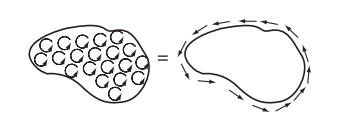
\includegraphics[width=8cm]{Electrodynamics/images/stokes.PNG}
\end{center}

Note that in this theorem, there is ambiguity in picking the direction of $d\vec{a}$ and also the direction to go in the loop integral on the right hand side. However, it suffices to simply be consistent! Use the right hand rule: if your fingers curl around in the direction that $d\vec{\ell}$ travels, your thumb marks the direction of $d\vec{a}$.

Similar to the fundamental theorem for gradients, this gives two important corollaries:

\begin{corollary}
    Surface integrals of curls are independent of the particular surface chosen. In particular
    \[\iint_{\mathcal{S}}(\nabla\times\vec{v})\cdot d\vec{a}\]
    depends only on $\partial\mathcal{S}$.
\end{corollary}

\begin{corollary}
    The integral of curls over a closed surface is equal to zero:
    \[\oiint (\nabla\times\vec{v})\cdot d\vec{a}=0.\]
\end{corollary}

\subsection{Integration by Parts}

Recall that the basic technique of integration by parts utilizes the product rule of derivatives:
\[\frac{d}{dx}(fg)=f\left(\frac{dg}{dx}\right)+g\left(\frac{df}{dx}\right).\]
Integrating both sides from $a$ to $b$ with respect to $dx$ gives
\[\left.fg\right\rvert_{a}^b=\int_a^bf\left(\frac{dg}{dx}\right)dx+\int_a^bg\left(\frac{df}{dx}\right)dx.\]
Rearranging gives
\[\boxed{\int_a^bf\left(\frac{dg}{dx}\right)dx=-\int_a^bg\left(\frac{df}{dx}\right)dx+\left.fg\right\rvert_a^b}.\]
Essentially, if you're integrating the product of one function $f$ and the \textit{derivative} of another function $g$, you can transfer the derivative from $g$ to $f$ at the cost of a boundary term of $fg$ on $\partial([a,b])=\{a,b\}$.

It turns out that you can exploit the product rules of vector calculus in the same way. For example, take the product rule for the divergence of a scalar times a vector:
\[\nabla\cdot(f\vec{v})=f(\nabla\cdot \vec{v})+\vec{v}\cdot(\nabla f).\]
By integrating over a volume, we can abuse Gauss' Law on the left hand side:
\[\iiint_{\mathcal{V}}\nabla\cdot(f\vec{v})d\tau=\iiint_{\mathcal{V}}f(\nabla\cdot \vec{v})d\tau+\iiint_{\mathcal{V}}\vec{v}\cdot(\nabla f)d\tau.\]
The left hand side reduces to
\[\oiint_{\partial\mathcal{V}}f\vec{v}\cdot d\vec{a},\]
so we can write
\[\boxed{\iiint_{\mathcal{V}}f(\nabla\cdot\vec{v})d\tau=-\iiint_{\mathcal{V}}\vec{v}\cdot(\nabla f)d\tau+\oiint_{\partial\mathcal{V}}f\vec{v}\cdot d\vec{a}}.\]
Notice how this has the same form as vanilla integration by parts: we can transfer a derivative (in this case a divergence) from $\vec{v}$ to $f$ (it turns into a gradient) at the cost of a boundary term.

It turns out that integration by parts is actually one of the most powerful tools in vector calculus; there are two other forms presented in the problem below:

\section{Curvilinear Coordinates}

\subsection{Spherical Coordinates}

Recall that instead of Cartesian coordinates, you can also label points in space using \vocab{spherical coordinates} $(r,\theta,\varphi)$. We use physics convention here, where $r=|\vec{r}|$ is the distance to the origin; $\theta$ is the \vocab{polar angle}, the angle between $\vec{r}$ and the $z$-axis; and $\varphi$ is the \vocab{azimuthal angle}, the angle around from the $x$-axis. 

We can easily relate these to Cartesian coordinates:
\[x=r\sin\theta\cos\varphi, \qquad y=r\sin\theta\sin\varphi, \qquad z=r\cos\theta.\]
It turns out that the unit vectors $\hat{r}$, $\hat{\theta}$, and $\hat{\varphi}$ form an orthonormal basis of $\mathbb{R}^3$. Hence you can express any vector $\vec{a}$ as
\[\vec{a}=a_r\hat{r}+a_\theta\hat{\theta}+a_\varphi\hat{\varphi}.\]
It is not too hard to check that
\[
\begin{cases}
\hat{r}=\sin\theta\cos\varphi\cdot \hat{x}+\sin\theta\sin\varphi\cdot\hat{y}+\cos\theta\cdot\hat{z},\\
\hat{\theta}=\cos\theta\cos\varphi\cdot\hat{x}+\cos\theta\sin\varphi\cdot\hat{y}-\sin\theta\cdot\hat{z},\\
\hat{\varphi}=-\sin\varphi\cdot\hat{x}+\cos\varphi\cdot\hat{y}.
\end{cases}
\]

However, there is a very important caveat about this coordinate system! The unit vectors $\hat{r}$, $\hat{\theta}$, and $\hat{\varphi}$ are associated with the \textit{particular point} $P$ that is chosen, and they change direction as $P$ moves around! Therefore, unlike $\hat{x}$, $\hat{y}$, and $\hat{z}$, these basis vectors are not constants. 

For example, do not combine the spherical coordinates of vectors associated with different points (e.g. if $\vec{a}$ and $\vec{b}$) are unit vectors pointing in opposite directions, even though $\vec{a}=\hat{r}$ in its own coordinate system and $\vec{b}=\hat{r}$ in its own coordinate system, we still have that $\vec{a}+\vec{b}=\vec{0}$, not $2\hat{r}$). 

In addition, you need to be careful with differentiating a vector in spherical coordinates, since the unit vectors themselves are functions of position, and need to be differentiated (e.g. $\partial \hat{r}/\partial \theta=\hat{\theta}$).  In addition, you cannot take $\hat{r}$, $\hat{\theta}$, or $\hat{\varphi}$ outside of an integral (e.g. as we did right after Definition \ref{defvolint} in the definition of the volume integral of a vector function).

Due to the setup of spherical coordinates, infinitesimal elements of length are
\[d\vec{\ell}=dr\cdot \hat{r}+rd\theta\cdot \hat{\theta}+r\sin\theta d\varphi\cdot \hat{\varphi}.\]
We call these respective small steps in the $\hat{r}$, $\hat{\theta}$, and $\hat{\varphi}$ directions $d\ell_r=dr$, $d\ell_\theta=rd\theta$, and $d\ell_\varphi=r\sin\theta d\varphi$. 

Similarly, the infinitesimal elements of volume are also different:
\[d\tau=d\ell_r d\ell_\theta d\ell_{\varphi}=r^2\sin\theta drd\theta d\varphi,\]
the product of the scalings $r$ and $r\sin\theta$ that we applied above to the $\hat{\theta}$ and the $\hat{\varphi}$ directions, respectively.

As you can probably imagine, the expression for surface elements is also different, but it's hard to give a general form since it depends on the orientation of the surface. In general, you can always directly analyze the geometry for any given case, but for some examples:
\begin{itemize}
    \item If $r$ is constant (e.g. integrating over a sphere), we have
    \[d\vec{a}=d\ell_\theta d\ell_\varphi\hat{r}=r^2\sin\theta d\theta d\varphi\hat{r}.\]
    \item If the surface lies in the $xy$ plane so that $\theta$ is constant, then
    \[d\vec{a}=d\ell_r d\ell_\varphi\hat{\theta}=rdrd\varphi\hat{\theta}.\]
\end{itemize}
Finally, we note that $r\in [0,\infty)$, $\varphi\in[0,2\pi]$, and $\theta\in[0,\pi]$.

\begin{example}
Find the volume of a sphere of radius $R$.
\end{example}

\begin{proof}[Solution]
Integrate
\begin{align*}
    V&=\iiint_{\mathcal{V}}d\tau=\int_{r=0}^R\int_{\varphi=0}^{2\pi}\int_{\theta=0}^\theta (r^2\sin\theta) d\theta d\varphi dr\\
    &=\left(\int_{0}^R r^2 dr\right)\left(\int_0^{2\pi} d\varphi\right)\left(\int_0^{\pi}\sin\theta d\theta\right)\\
    &=\left(\frac{R^3}{3}\right)(2\pi)(2)=\frac{4}{3}\pi R^3,
\end{align*}
as expected.
\end{proof}

Alright, that finishes a discussion of the \textit{geometry} of spherical coordinates. However, we still need to translate all the vector derivatives we've already discussed. Brute forcing thing would be quite hard, but Appendix describes a much more efficient method, which happens to treat all coordinate systems at once (I haven't taken notes for this, but maybe will in the future).

In any case, let's cut to the chase and just give the formulas:

\begin{proposition}[Vector derivatives in spherical coordinates]
    \begin{itemize}
        \item[]
        \item Gradient:
        \[\nabla T=\frac{\partial T}{\partial r}\hat{r}+\frac{1}{r}\frac{\partial T}{\partial\theta}\hat{\theta}+\frac{1}{r\sin\theta}\frac{\partial T}{\partial\varphi}\hat{\varphi}.\]
        \item Divergence:
        \[\nabla\cdot\vec{v}=\frac{1}{r^2}\frac{\partial}{\partial r}(r^2v_r)+\frac{1}{r\sin\theta}\frac{\partial}{\partial\theta}(\sin\theta v_\theta)+\frac{1}{r\sin\theta}\frac{\partial v_\varphi}{d\varphi}.\]
        \item Curl:
        \begin{align*}
            \nabla\times\vec{v}&=\frac{1}{r\sin\theta}\left[\frac{\partial}{\partial\theta}(\sin\theta v_\varphi)-\frac{\partial v_\theta}{\partial \varphi}\right]\hat{r}+\frac{1}{r}\left[\frac{1}{\sin\theta} \frac{\partial v_r}{\partial \varphi}-\frac{\partial}{\partial r}(rv_\varphi)\right]\hat{\theta}\\
            &+\frac{1}{r}\left[\frac{\partial}{\partial r}(rv_\theta)-\frac{\partial v_r}{\partial \theta}\right]\hat{\varphi}.
        \end{align*}
        \item Laplacian:
        \[\nabla^2 T=\frac{1}{r^2}\frac{\partial}{\partial r}\left(r^2\frac{\partial T}{\partial r}\right)+\frac{1}{r^2\sin\theta}\frac{\partial}{\partial \theta}\left(\sin\theta\frac{\partial T}{\partial \theta}\right)+\frac{1}{r^2\sin^2\theta}\frac{\partial^2T}{\partial \varphi^2}.\]
    \end{itemize}
\end{proposition}

\subsection{Cylindrical Coordinates}

Another method of labeling $\mathbb{R}^3$ is using \vocab{cylindrical coordinates} $(s,\varphi,z)$; where we simply project $P$ down to the $xy$-plane and assign polar coordinates $(s,\varphi)$ to the projection, then let $z$ be the height off the $xy$-plane along the $z$-axis. These relate by
\[x=s\cos\varphi,\qquad y=s\sin\varphi, \qquad z=z.\]
The unit vectors can be written as
\[\begin{cases}
\hat{s}= \cos\varphi\hat{x}+\sin\varphi\hat{y},\\
\hat{\varphi}=-\sin\varphi\hat{x}+\cos\varphi\hat{y},\\
\hat{z}=\hat{z}.
\end{cases}\]
Infinitesimal elements of length are
\[d\vec{\ell}=ds\cdot\hat{s}+sd\varphi\cdot \hat{\varphi}+dz\cdot\hat{z},\]
where the respective small steps in the $\hat{s}$, $\hat{\varphi}$, and $\hat{z}$ directions are $d\ell_s=ds$, $d\ell_\varphi=sd\varphi$, and $d\ell_z=dz$.

Hence, the volume element is
\[d\tau=sdsd\varphi dz.\]
Finally, note that $s\in[0,\infty)$, $\varphi\in[0,2\pi]$, and $z\in(-\infty,\infty)$.

\begin{proposition}[Vector derivatives in cylindrical coordinates]
    \begin{itemize}
        \item[]
        \item Gradient:
        \[\nabla T=\frac{\partial T}{\partial s}\hat{s}+\frac{1}{s}\frac{\partial T}{\partial\varphi}\hat{\varphi}+\frac{\partial T}{\partial z}\hat{z}.\]
        \item Divergence:
        \[\nabla\cdot\vec{v}
        =\frac{1}{s}\frac{\partial}{\partial s}(sv_s)+\frac{1}{s}\frac{\partial v_\varphi}{\partial\varphi}+\frac{\partial v_z}{\partial z}.\]
        \item Curl:
        \[\nabla\times \vec{v}=\left(\frac{1}{s}\frac{\partial v_z}{\partial\varphi}-\frac{\partial v_\varphi}{\partial z}\right)\hat{s}+\left(\frac{\partial v_s}{\partial z}-\frac{\partial v_z}{\partial s}\right)\hat{\varphi}+\frac{1}{s}\left[\frac{\partial}{\partial s}(sv_\varphi)-\frac{\partial v_s}{\partial\varphi}\right]\hat{z}.\]
        \item Laplacian:
        \[\nabla^2 T=\frac{1}{s}\frac{\partial}{\partial s}\left(s\frac{\partial T}{\partial s}\right)+\frac{1}{s^2}\frac{\partial^2T}{\partial\varphi^2}+\frac{\partial^2T}{\partial z^2}.\]
    \end{itemize}
\end{proposition}

\section{The Dirac Delta Function}

\subsection{The Divergence of $\hat{r}/r^2$}

Major apparent paradox: consider 
\[\vec{v}=\frac{1}{r^2}\hat{r}.\]
This function has all arrows pointing outwards; if any vector function would have positive divergence, this is it! Yet, if we calculate the divergence anywhere, we get
\[\nabla\cdot\vec{v}=\frac{1}{r^2}\frac{\partial}{\partial r}\left(r^2\cdot\frac{1}{r^2}\right)=0.\]
What's going on? In fact, it gets even worse if we try applying the divergence theorem. Integrating over a sphere $\mathcal{V}$ of radius $R$ centered at the origin, the surface integral is
\begin{align*}
\oiint_{\partial \mathcal{V}}\vec{v}\cdot d\vec{a}&=\oiint_{\partial\mathcal{V}}\left(\frac{1}{R^2}\hat{r}\right)\cdot (R^2\sin\theta d\varphi d\theta\cdot \hat{r})\\
&=\int_0^\pi \int_0^{2\pi} \sin\theta d\varphi d\theta\\
&=2\pi\cdot\int_0^\pi\sin\theta d\theta=4\pi.
\end{align*}
And yet
\[\iiint_{\mathcal{V}}(\nabla\cdot\vec{v}) d\tau=0,\]
so what's going on? Are we to believe that the divergence theorem is false?

The solution is where $r=0$: the divergence must blow up there. It turns out that $\nabla\cdot \vec{v}$ has the wild property that it vanishes everywhere except one point, yet its integral over any volume including that point is $4\pi$. No ordinary function behaves like this, but it turns out we've stumbled on what is known to physicists as the \vocab{Dirac delta function}.

\subsection{The One-Dimensional Dirac Delta Function}

\begin{definition}
    The \vocab{one-dimensional Dirac delta function}, $\delta(x)$ can be pictured as an infinitely high, infinitesimally narrow ``spike" at the origin, with area 1. Indeed,
    \[\delta(x)=\begin{cases}
    0 & \text{if }x\neq 0\\
    \infty & \text{if }x=0
    \end{cases}\]
    and
    \[\int_{-\infty}^\infty\delta(x)dx=1.\]
    If $x$ has units meters, then $\delta(x)$ has units $(\text{meters})^{-1}$.
\end{definition}

In reality, $\delta(x)$ is not a function since its value at $0$ isn't finite: instead, it's a \vocab{generalized function}, or \vocab{distribution}. It is a \textit{limit} of a \textit{sequence} of functions, say rectangles with height $n$ and width $1/n$, or isosceles triangles of height $n$ and base $2/n$, centered at the origin (as $n\to\infty$).

Note that for an ordinary (continuous) function $f$, we have
\[f(x)\delta(x)=f(0)\delta(x),\]
as their product is 0 whenever $x\neq 0$. Hence
\[\int_{-\infty}^\infty f(x)\delta(x)dx=f(0)\int_{-\infty}^\infty\delta dx=f(0).\]
Under an integral, the delta function ``picks out" the value of $f(x)$ at $x=0$.

We can shift the spike anywhere with $\delta(x-a)$. Then
\[\boxed{\int_{-\infty}^{\infty}f(x)\delta(x-a)dx=f(a)}.\]
This is so important that I've boxed it.

\begin{example}
Evaluate the integral
\[\int_0^3x^3\delta(x-2)dx.\]
What if the upper bound was 1 instead?
\end{example}

\begin{proof}[Solution]
The delta function picks out the value of $x^3$ at $2$, which is $\boxed{8}$. If the upper bound was 1 instead, we wouldn't catch the spike since $2\not\in[0,1]$; hence the integral would be 0.
\end{proof}

So in fact, you should really think of the delta function as something that is \textbf{always intended for use under and integral sign}. In particular, given two expressions $D_1, D_2$ involving delta function, we say that they're considered equal if
\[\int_{-\infty}^\infty f(x)D_1(x)dx=\int_{-\infty}^\infty f(x)D_2(x)dx\]
for \textit{all} functions $f(x)$.

Note that this is because if $D_1$ and $D_2$ were to differ around the neighborhood of some point $x=x'$, then we could just pick $f(x)$ to have a large spike at $x'$, and then the integrals wouldn't be equal anymore.

By $u$-substitution, it can also be shown that
\[\delta(kx)=\frac{1}{|k|}\delta(x).\]
This makes sense, as the factor of $k$ makes it so that you're ``passing through" $\RR$ $k$ times as fast, so you expect to pick up $\frac{1}{|k|}$ as much of it.

\subsection{The Three-Dimensional Delta Function}

If we write $\vec{r}=x\hat{x}+y\hat{y}+z\hat{z}$, then we can generalize:

\begin{definition}
    The \vocab{three-dimensional Dirac delta function} is defined as
    \[\delta^3(\vec{r})=\delta(x)\delta(y)\delta(z).\]
    It is zero everywhere except the origin, where it blows up, and its volume integral is 1:
    \[\iiint_{\mathbb{R}^3}\delta^3(\vec{r})d\tau=\int_{-\infty}^\infty\int_{-\infty}^\infty\int_{-\infty}^\infty\delta(x)\delta(y)\delta(z)=1.\]
\end{definition}

In addition, we have that

\[\boxed{\iiint_{\mathbb{R}^3}f(\vec{r})\delta^3(\vec{r}-\vec{a})d\tau=f(\vec{a})}.\]

To resolve the paradox at the start of this section, we can note that
\[\nabla\cdot\left(\frac{\hat{r}}{r^2}\right)=4\pi\delta^3(\vec{r}).\]
More generally,
\[\boxed{\nabla\cdot\left(\frac{\hat{\scr}}{\scr^2}\right)=4\pi\delta^3(\vec{\scr})},\]
where, recall, $\vec{\scr}=\vec{r}-\vec{r'}$ for some source $\vec{r'}$. Also, since $\nabla\left(\frac{1}{\scr}\right)=-\frac{\vec{\scr}}{\scr^2}$, we have that its Laplacian is
\[\nabla^2\frac{1}{\scr}=-4\pi\delta^3(\vec{\scr}).\]

\section{The Theory of Vector Fields}

